% Possible background additions:
% Positive/Negative examples ILASP.
% Semantic parsing maybe.

% Add a box plot somewhere


% TODO: Alessandra feedback: use running examples because it's easier to understand that way
% TODO: Alessandra feedback: do comparison with semantic entailment if it is
\chapter{Solving NLP Tasks Logically}
\label{solving-nlp-tasks-logically}


Logical representations have an important place in the Natural Language Processing field.
Semantic parsing \cite{RefWorks:RefID:28-jurafsky2014speech} is a famous task that aims to convert a natural language input that captures the meaning of that input.
After all, having a sentence in a logical form allows reasoning about it to form new conclusions.

However, in this chapter, the logic is used in a slightly unconventional manner for NLP.
It is an intermediate representation for a sequence-to-sequence problem where it captures only the syntax of the text rather than its meaning.
The current state of the art approach for sequence-to-sequence problems, such as language translation, uses transformers. 
Nevertheless, seq2seq transformers would perform poorly with available datasets for the two problems tackled in this chapter.
The datasets consisting of ~100 examples are too small for a model with billions of parameters to be able to generalise.
% INSERT Imdb dataset reference 
Transformer fine-tuning is usually done on tens of thousands of examples, such as the IMDB Movie Reviews dataset. \\
% INSERT reference second year notes.
On the other hand, logic-based learning systems can generalise well from a tiny number of examples, making them suitable for the problems presented in this chapter. \\


In this chapter, the following topics are presented:
\begin{itemize}
    \item Introduction of atomisation and generalisation tasks
    \item A logical approach to solving the generalisation task.
    \item A logical approach to solving the atomisation task.
    \item Implementation details for solving these two problems.
    \item Evaluation of the two methods.
\end{itemize}



% TODO: Alessandra feedback: add more introduction, namely the drawing in alessandra-feedback-diagram - one box is for the atomiser (symbolic atomisation transformer), another one for generalisation - they work on sentences to sentences
% TODO: Alessandra feedback: go into how both atomisation and generalisation works briefly
% TODO: Alessandra feedback: add more introduction, namely the drawing in alessandra-feedback-diagram

% From what I understood Ale's feedback is decided on the Nuri's paper - if there is time look into his papers for inspiration
 
\section{Sequence2Sequence Tasks}

The two tasks that have been tackled using logic based learning approach are \textbf{sentence} \textbf{atomisation} and \textbf{generalisation}.

The former converts a declarative sentence into one or more \textbf{atomic sentences}, while the latter converts an \textbf{atomic sentence} into one or more \textbf{concept sentences}.

% TODO: Alessandra feedback: no need for a subsection. Merge with the previous one
\subsection{Sentence Type Definitions}
\label{sentence-type-definitions}

\textbf{Atomic Sentence:} A sentence that cannot be decomposed into multiple valid sentences. \\
% TODO add reference %
Note that this is equivalent to the definition used in logic.
However, the sentence structure considered in this project is often much more complex than the one considered in logic.\\
% INSERT insert simple predicates definition reference %
An \textbf{atomic sentence} should only contain simple predicates, eliminating compound and complete predicates from a sentence.


\textbf{Concept Sentence:} A syntactic generalisation of an atomic sentence, which satisfies the following three conditions:
\begin{enumerate}
% TODO: Alessandra feedback: valid -> syntactically well-formed -> give examples for what it means for a sentence to be syntactically well-formed
    \item It is a valid sentence in its own right.
    \item True if the atomic sentence is.
    \item Obtained only through syntactic manipulation of an atomic sentence, a result of modifying the syntax tree of the sentence.
\end{enumerate}

% TODO: Alessandra feedback: argue that concept sentence is any syntactically well formed substring of an atomic sentence.
Concept sentences are sometimes referred to as \textbf{(syntactic) generalisations} of a sentence in this report.


\begin{example}
Splitting a given sentence into all its concepts sentences.

Starting from the sentence:  
\begin{verbatim}
The batter caught the ball in the air and sent it into the left field.
\end{verbatim}
we can extract the following atomic sentences: 
\begin{verbatim}
The batter made contact with the ball in the air. 
The batter sent it into the left field.
\end{verbatim}
From these two sentences, we can obtain four concept sentences: 
\begin{verbatim}
The batter made contact with the ball in the air.
The batter made contact with the ball.
The batter sent it into the left field.
The batter sent it into the field.
The batter sent it.
\end{verbatim}

\end{example}

% TODO: Alessandra feedback: no need for a subsection. Merge with the previous one
\subsection{Purpose of the Tasks}

The two tasks mentioned are a part of the Concept Bottleneck pipeline discussed in greater detail in Chapter \ref{concept-bottleneck-pipeline}
These two tasks are used in sequence as a replacement for the extraction part of the original CoDEx (Concept Discovery and Extraction) pipeline \ref{inherited-work}.

The reason the project aims to extract all concept sentences from a particular sentence is two-fold:
\begin{enumerate}
    \item Concept sentences help associate differently worded explanations of the same concept.
    \item The final generated sentences are immediately usable for explanations.
\end{enumerate}

% TODO: Alessandra feedback: add part 2 of the diagram from the introduction but now show the syntactic parse trees to showcase what we are doing in this part
% TODO: Alessandra feedback: talk about the definition of the learning task associated with the background.
% TODO: Alessandra feedback: make background/language_bias \paragraph or something similar so that they don't appear in the table of contents
\section{Solving Concept Generalisation}
\label{solving-generalisation-task}

\subsection{Logical Encoding}
\label{logical-encoding}

In this subsection, we showcase how the example sentences are encoded logically and the pipeline used at test time to generate solutions.
All encodings are compatible with the Answer Set Programming \cite{RefWorks:RefID:1-lifschitz2008answer} paradigm.
The solution learning is described in the following subsection (\ref{encoding-the-learning-task}), which relies on the encodings presented in this subsection. 


A solution to the \textbf{concept generalisation} task is learned using the Inductive Logic Programming tool ILASP \cite{RefWorks:RefID:18-law2020ilasp}.

\subsubsection{Encoding the Example Premise}

% TODO: delete this because it is discussesed in the implementation
\textbf{Generalisation} examples consist of a given sentence followed by one to many sentences, which are ways in which the provided sentence can be generalised/atomised.
For instance, here is a possible \textbf{generalisation} example:
\begin{verbatim}
"It was a fast ball.", "It was a ball. It was a fast ball."
\end{verbatim}


We first need to define a way to convert the sentences into a logical representation that we could use to reason about the sentence structure.
Ideally, a sentence representation should satisfy the following criteria:
\begin{itemize}
    \item Word dependency capture --- The representation should capture dependencies between words to determine whether a word is crucial to the meaning of a sentence.
    \item Similar meaning $\rightarrow$ similar encoding --- Slight word variations such as words replaced by synonyms should be encoded similarly. The task becomes easier for the learner when the words with the same meaning are captured by the exact representation.
    \item Compactness --- Smaller representations are quicker to process. 
    \item Domain independence --- We want to apply the generalisation task in various domains, so the representation should not contain domain-specific information.
    \item Interpretability --- It should be clear what the representation encodes. We can translate the learned ILASP solution into English if the predicates are interpretable. Hence, we can verify whether the system learned spurious correlations or valuable rules.
    \item Reconstuctability --- One should be able to reconstruct a sentence as the final output of the task needs to be a correct sentence.
\end{itemize}


% INSERT word2vec reference
A common approach to encoding a sentence involves using dense-vector contextualised embeddings of words, such as the ones produced by Word2vec.
Dense-vector embeddings are practical because they are compact and tend to capture the semantics of words (i.e. map similar words to similar value embeddings).
Transformers improve upon these embeddings by using the self-attention mechanism to provide an even better representation of a sentence.

However, dense-vector embeddings are not interpretable, making them difficult to use with our problem. 
The learning approach that we have used follows a similar idea of trying to capture semantic relationships within a sentence.
We utilise the \textbf{dependency parse tree} as a basis for the \textbf{generalisation} task as it captures syntactic relationships between words.
% INSERT reference NLP notes
Note that the syntactic relationships captured approximate the semantic relationships between words.
In addition, words themselves are put into logical predicates, making the sentences reconstructible.

The dependency tree gives rise to the following predicates:
\begin{verbatim}
    dep(l, token1, token2).
    root(token).
    token(token, string).
\end{verbatim}

It represents that there exists an arc from \verb_token1_ to \verb_token2_ with label \verb+l+ which are converted back to string form with \verb_token_ predicate.
In addition, \verb_root_ encodes which token is the root of the sentence.

\begin{example}
\label{logical-encoding-example}
Encoding \textit{he threw a fast ball}, with a dependency graph shown in \ref{example-dependency-graph}:
\begin{enumerate}
    \item Convert each token in the tree to a logical form
    \begin{verbatim}
        token(tok0, "he").
        token(tok1, "threw").
        token(tok2, "a").
        token(tok3, "fast").
        token(tok4, "ball").
    \end{verbatim}
    \item Convert arcs and roots of the tree to predicates:
    \begin{verbatim}
        root(tok1).
        dep(nsubj, tok1, tok0).
        dep(dobj, tok1, tok4).
        dep(det, tok4, tok2).
        dep(amod, tok4, tok3).
    \end{verbatim}
\end{enumerate}
\end{example} 

\begin{figure}[h]
\caption{Dependency graph of \emph{He threw a fast ball.}}
\centering
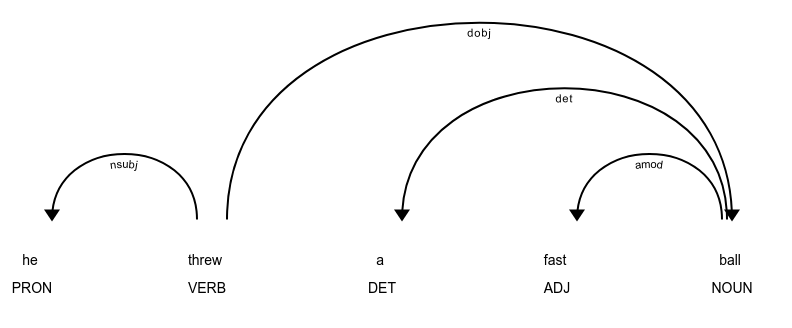
\includegraphics[width=\textwidth]{solving-nlp-tasks-logically/example_dependency_tree.png}
\label{example-dependency-graph}
\end{figure}

Reflecting on the criteria outlined at the start of the section, we can see that it is mainly satisfied by the encoding. 
Even the similar meaning $\rightarrow$ similar encoding is captured somewhat in the context of this problem.
The two sentences which only differ by one synonym would be identically represented by the \verb_dep_ predicates, resulting in any model treating them similarly.
For example, the sentences:
\begin{verbatim}
    The batter hit the ball. The hitter hit the ball.
\end{verbatim}
would have the equal \verb_dep_ predicate representation. 
However, the sentences:
\begin{verbatim}
    The batter hit the ball. The ball was hit by the batter.
\end{verbatim}
would not have similar representations.
This representation drawback did not end up being a hurdle for the current dataset.

\subsubsection{Encoding the Example Target}
\label{encoding-the-example-target}


After the example observation, it became clear that concept sentences contained only the words used in the premise.
We could model the problem in this section as to whether or not we want to include the word in a concept sentence.
That goal is denoted with a predicate:
\begin{verbatim}
   in_generalised_sent(t).
\end{verbatim}
which represents that a token \verb+t+ is included in the concept sentence.
The possibility of multiple concept sentences existing is modelled using multiple answer sets.
\begin{example}
\label{example-encoding-target}
Encoding \textit{he threw a ball} as a generalisation of \textit{he threw a fast ball}:

From the previous example (\ref{logical-encoding-example}), we have:
\begin{verbatim}
    token(tok0, "he"). token(tok1, "threw"). token(tok2, "a"). 
    token(tok3, "fast"). token(tok4, "ball").
\end{verbatim}
So, we the example target is encoded as:
\begin{verbatim}
    in_generalised_sent(tok0). in_generalised_sent(tok1). 
    in_generalised_sent(tok2). in_generalised_sent(tok3). 
\end{verbatim}

\end{example}

\subsection{Encoding the Learning Task}
\label{encoding-the-learning-task}

Learning a solution with ILP is different from determining a solution with Deep Learning.
% INSERT reference to KR notes
Inductive Logic Programming uses a different level of knowledge representation commitment than Deep Learning.
Deep Learning approaches do not give any inductive bias to a machine. 
The model must learn how to solve the problem from the data only. \\
On the other hand, Inductive Logic Programming requires more human-generated knowledge representation.
In particular, the logical structure is encoded to the learner, which is encouraged to find all possible theories within that structure and return the best one. 
Because of this property, the Inductive Logic Programming paradigm can incorporate existing knowledge into the final solution, making the task easier to solve.

The following subsection demonstrates how the \textbf{generalisation} task has been solved with ILASP \cite{RefWorks:RefID:18-law2020ilasp}, a state-of-the-art ILP system.

% TODO: Alessandra feedback: describe a problem with learner first before going into a hand-crafted solution (after learning)
% Argue that a hand-crafted solution should be something a human engineered ground truth model

\subsubsection{Background Knowledge Construction}

Here is the background knowledge used for the \textbf{generalisation} task.
\begin{verbatim}
token(T) :- root(T).
token(T) :- dep(_, T, _).
token(T) :- dep(_, _, T).
label(L) :- dep(L, _, _).

% there must be a token in any concept sentence
:- #count{T : in_generalised_sent(T)}0.
\end{verbatim}
The first four rules define unary predicates used as types in language bias, while the final rule encodes that a generalised sentence should not be empty.

\subsubsection{Language Bias}

The construction of the language bias was done by first designing a hand-crafted ASP solution that tackles the task well, followed by encoding all predicates used in that solution to ILASP.
The hand-crafted solution helps find the structure logical structure the learner should know.
ILASP should then be able to find a better solution within those constraints.


% TODO: Alessandra feedback: Justify a 0 1 boundary
The problem is modelled as a choice of whether a particular token (word) should always be included or sometimes be included in the solution, which the following types of rules can represent.
\begin{verbatim}
in_generalised_sent(T) :- ...
0 {in_generalised_sent(T) } 1 :- ...
\end{verbatim}

This gives rise to the following language bias:
\begin{verbatim}
#modeh(in_generalised_sent(var(token))).
#modeha(in_generalised_sent(var(token))).

#modeb(in_generalised_sent(var(token))).
#modeb(root(var(token))).
#modeb(dep(const(label), var(token), var(token)), (positive)).

#bias("
% Only allow rules 0 { in_generalised_sent(V1) } 1.
% Eliminates all generated rules that where lhs of 
% the curly brace is >= 1.
:- in_head(_), lb(1).
").

% Disallow 2+ in_generalised_sent predicates occurring within {}.
#disallow_multiple_head_variables.

\end{verbatim}

% TODO: Alessandra feedback: what would happen if we only had #pos examples.
% TODO: Alessandra feedback: Argue that the size is because of the number of constants that we have. 
\subsubsection{Example Encoding}
\label{example-encoding}

As mentioned, \textbf{generalisation} examples consist of a given sentence followed by 1 to many concept sentences.
We need to convert those representations into ILASP examples.
% INSERT: refer to background where a more formal definition is provided %
ILASP allows defining two types of examples as outlined more formally in \ref{examples-in-ilasp}.
\begin{itemize}
    \item positive (\verb_#pos_) - an example which should be by at least one answer set.
    \item negative (\verb_#neg_) - an example that any answer set should not extend.
\end{itemize}

Ideally, we want the solution learned by ILASP to produce the number of answer sets equal to the number of generalisations.
Using these two constructs, we can define that we want exactly one answer set for each possible generalisation. \\
It is done by creating a positive example for each sentence we wish to produce. 
In addition, a negative example is produced with the \verb_goal_ predicate in the exclusion for each text sentence example.
The \verb_goal_ predicate, defined only in the contexts of negative examples, is true if \verb+in_generalised_sent+ atoms correspond precisely to a positive example.


\begin{example}
Generating ILASP-compatible generalisation examples for \textit{"He threw a fast ball.", "He threw a ball. He threw a fast ball."}

% INSERT reference to previous section %
1. Convert the premise sentence to logical form, as shown in example \ref{logical-encoding-example}.

2. For each possible generalisation, create a positive example. The context consists of predicates produced in step 1, while the inclusion/exclusion of appropriate \verb+in_generalised_sent+ tokens (example \ref{example-encoding-target}). The concept sentence \textit{He threw a ball.} yields the following example:
\begin{verbatim}
#pos(example_id@noise_penalty,
{in_generalised_sent(tok0), in_generalised_sent(tok1), 
 in_generalised_sent(tok2), in_generalised_sent(tok4), 
 in_generalised_sent(tok5)},
{in_generalised_sent(tok3)}, % tok3 = "fast"
{
% all the predicates generated in step 1
}).
\end{verbatim}

3. The negative example is generated as follows:
\begin{verbatim}
#neg(example_id@noise_penalty,
{ },
{ goal },
{
% all the predicates generated in 1)

% He threw a fast ball.
goal :- in_generalised_sent(tok0), in_generalised_sent(tok1), 
        in_generalised_sent(tok2), in_generalised_sent(tok3), 
        in_generalised_sent(tok4), in_generalised_sent(tok5).
% He threw a ball.
goal :- in_generalised_sent(tok0), in_generalised_sent(tok1), 
        in_generalised_sent(tok2), in_generalised_sent(tok4), 
        in_generalised_sent(tok5)}, not in_generalised_sent(tok3).
}).
\end{verbatim}
\end{example}

All of the examples constructed have a \verb+noise_penalty=1+ as the \textbf{concept generalisation} examples may be noisy.


% TODO: Alessandra feedback: scaling up should be a separate section
\subsection{Managing Learning Scalability Constraints}

% INSERT reference for this. %
A considerable challenge with logic based learning systems, such as ILASP, is a lack of scalability when dealing with large scale AI problems compared to other forms of machine learning. \\
For the \textbf{generalisation} task, two challenges needed to be mitigated: 
\begin{itemize}
    \item Lack of scalability w.r.t size of the hypothesis space -- This issue arises due to ILASP enumerating search space $S_M$ in full before finding a solution.
    \item Extreme RAM consumption during task solving.
\end{itemize}

\subsubsection{Reducing the hypothesis space size}
\label{reducing-the-hypothesis-space-size}

For example, consider the following simplified language bias definition:
\begin{verbatim}
#modeh(in_generalised_sent(var(token))).
#modeb(in_generalised_sent(var(token))).
#modeb(root(var(token))).
#modeb(dep(const(label), var(token), var(token))).

... all the constant definitions ...
\end{verbatim}

% INSERT Might be benficial to include a table how each rule reduced the search space size.

It took over 13 hours to generate an entire search space on a machine with an Intel Core i7 10510U 1.80GHz / 4.90GHz processor and 16 GiB of RAM.

FastLAS \cite{RefWorks:RefID:19-law2020fastlas:} is a system designed to alleviate this particular constraint, but it can only deal with a restricted version of the learning task.
Its inability to produce a solution with multiple answer set made it inapplicable for the current problem.

% INSERT reference to Mark's website
The scalability issue was instead tackled using meta-level definitions of the hypothesis space, which allow much greater flexibility than simple \textit{modeb}, \textit{modeh} statements. 
They allow constraining how rules are generated using ASP syntax, removing rules that we do not want as a part of the learned solution.
We always want to remove the rules whose body could never be satisfied.

Here are some examples of they are utilised to restrict the search space presented in this section:
\begin{verbatim}
% Idea #1: Dep represents an arc in a tree. This allows 
% cutting out rules which are impossible to be satisfied.
    
% It is impossible to have more than 1 root per example.
:- #count{T : body(root(T))} > 1.

% Trees cannot have a relation to itself.
:- body(dep(_, X, X)).
:- body(naf(dep(_, X, X))).

% A tree is not symmetric.
:- body(dep(_, X, Y)), body(dep(_, Y, X)).

% No dependency can go to the root
:- body(root(X)), body(dep(_, _, X)).

% Idea #2: Only allow two dep rules to occur in a body
% under certain conditions. 

% Pairs of dependency tags which can co-occur.
% Much smaller set of all possible pairs.
dep_chain(prep, pobj).
dep_chain(pobj, amod).
...

% Allow any rule with at most one dep predicate
allowed_dep_rule :- #count{L, V4, V5 : body(dep(L, V4, V5))} <= 1.
% Allow rule with two dep predicates if it is labels are white-listed
% by dep_chains and tokens are chained too.
allowed_dep_rule :- body(dep(L1, _, V2)), body(dep(L2, V2, _)), 
                    dep_chain(L1, L2), 
                    #count{L, V4, V5 : body(dep(L, V4, V5))} = 2.

:- not allowed_dep_rule.

% Idea 3: Remove rules that where simpler rules would suffice.

% Rule with root(V3) where V3 is not used in any dep is not needed.
% This predicate is trivially satisfied since every sentence has a 
% root.
:- body(root(X)), not body(dep(_, X, _)), not body(dep(_, _, X)), 
   body(dep(_, _, _)).

% If we have a in_generalised_sent predicate there must be some logic 
% related to it.
% This predicate is trivially satisfied otherwise, since the 
% background requires that at least one must always exist.
:- body(in_generalised_sent(X)), not body(dep(_, X, _)), 
   not body(dep(_, _, X)).


\end{verbatim}

These modifications allowed the search space generation times to take less than a minute, starting from over 13 hours.
The final search space consisted of only 3652 rules.


% TODO: Alessandra feedback: avoid using OOM acrynoym - replace with out-of-memory/lack of memory
\subsubsection{Avoiding OOM Errors}
\label{avoiding-oom-errors}

ILASP memory consumption is drastic even for the simpler of the two tasks solved logically.
% INSERT memory graph drawn on batch machine over time for generalisation.
The memory consumption graph over time is outlined in \ref{generalisation-memory-graph}.
As seen in the plot, the graph is at around 15 GB of RAM at about 15-hour mark.
So, to prevent the usual 16 GB machines from going out of memory, the execution is terminated after 15 hours, and the best solution found until that point is returned.
This technique prevents the ILASP process from exceeding the memory limit while returning a high-quality result.

% INSERT reference to PyLASP doc
The aforementioned ILASP behaviour modification is possible through the use of PyLASP scripts.

\begin{figure}[h]
\caption{Comparison of the ILASP solution performance and memory consumption over time. A lower ILASP score corresponds to a better solution.}
\centering
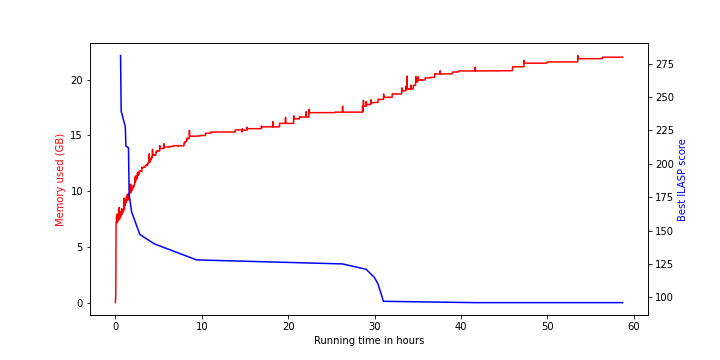
\includegraphics[width=\textwidth]{solving-nlp-tasks-logically/generalisation_memory_vs_best_score.png}
\label{generalisation-memory-graph}
\end{figure}

\subsection{Final Solution}

The final solution is obtained by running ILASP with background, language\_bias, examples and the custom PyLASP script.
In addition, all ILASP tasks were run with the \verb+--restarts+ flag, which can help reduce the running time of a program.

% INSERT reference to evaluation part of this section
The results of the performance of the \textbf{generalisation} task can be found in \ref{concept-generalisation-results}.


% TODO: Alessandra feedback: argue that atomistaion is a 3-step process - generate logical form + apply rules + reconstruct the data
% TODO: Alessandra feedback: add diagram with dependency trees - alessandra feedback-diagrams.png has a sketch

% TODO: Alessandra feedback: add part 1 of the diagram from the introduction but now show the syntactic parse trees to showcase what we are doing in this part
% TODO: Alessandra feedback: argue why the atomisation task is harder than the generalisation
\section{Solving Atomisation Task}
\label{solving-atomisation-task}

The solution to the atomisation task has only been hand-crafted rather than learned.
This section will highlight the idea behind the hand-crafted solution and demonstrate that ILASP is currently not scalable enough to learn a solution that is at least as good as the hand-crafted one.

\subsection{Shared Encoding Logic with Generalisation}

Due to the domain similarity of the two tasks, almost the entire Logical Encoding subsection (\ref{logical-encoding}) is fully applicable for the \textbf{atomisation} task with the following caveat:
\begin{itemize}
    % INSERT reference
    \item Encoding the Learning Target (\ref{encoding-the-example-target}) --- The goal for the \textbf{atomisation} task is denoted with \verb+in_atomised_sent+.
\end{itemize}

% TODO: Alessandra feedback: summarise the rules in English first before encoding them symbolically
% TODO: Alessandra feedback: include a table with two columns (predicate name, description) before which highlight what each of the predicates mean (so candidate_start is ...)
\subsection{Hand-crafting the Atomisation Solution}
\label{hand-crafting-the-atomisation-solution}

Consider the following two sentences and the desired atomisation, as well as the dependency graphs of the premises (\ref{atomisation-examples}):
\begin{lstlisting}
the batter swung and the ball landed 
  $\rightarrow$ the batter swung. the ball landed.
the batter swung and missed 
  $\rightarrow$ the batter swung. the batter missed.
\end{lstlisting}

% TODO Alessandra feedback: argued that there can only be one root in a dependency parse tree.

\begin{figure}[h]
\caption{Dependency graph of two sentences which need to be atomised}
\centering

\includegraphics[width=\textwidth]{solving-nlp-tasks-logically/dependency-graph-one-subj.png}

\includegraphics[width=\textwidth]{solving-nlp-tasks-logically/dependency-graph-two-subj.png}
\label{atomisation-examples}
\end{figure}

The graph illustrates that the terms on both ends of the \verb_conj_ tag should appear in separate sentences. 
Determining splitting tags, tags whose words should be in distinct subsets, is the core idea of the hand-crafted solution.
The words at the edges of these tags become starting points for generating sentences, which are constructed by adding tokens related to current \verb+in_atomic_sent+ tokens.

Following such an approach, the following set of rules was constructed:
\begin{lstlisting}

% Capture tokens at the end of a splitting tag
candidate_start(T) :- splitting_tag(C), dep(C, T, _).
candidate_start(T) :- splitting_tag(C), dep(C, _, T).

% Start splitting tags. Splitting tags must be a part of 
% distinct atomic sentences.
1 { in_atomic_sent(T) : candidate_start(T) } 1.

% Root should be a starting point if there are no 
% splitting tags.
in_atomic_sent(T) :- root(T), not candidate_start(_).

% Tags linking tokens that should be in distinct answer 
% sets, each with an example which sparked the choice:

% The batter swung therefore it is a strike.
% $\rightarrow$ The batter swung. It is a strike.
splitting_tag(ccomp).
% The batter did not swing so it was a ball.  
% $\rightarrow$ The batter did not swung. It is a ball.
splitting_tag(advcl).
% The batter swung the bat but missed the ball.
% $\rightarrow$ The batter swung the bat. The batter missed the ball.
splitting_tag(conj).
% The batter hit the ball in play where it was caught 
% mid air by a defender.
% $\rightarrow$ The batter hit the ball in play. It was caught mid air by a defender.
splitting_tag(relcl).



% Include all incoming relationships except candidate_starts. 
% This allows us to reach the predicate of the current atomic sentence.
% Atulve's ball was fast and good.
in_atomic_sent(T) :- dep(_, T, T2), in_atomic_sent(T2), not candidate_start(T).


% Incoming relationships first conjunct (conj) should also be included for the second one.
% This holds for conj only. The clauses tend to be self-sufficient.
% Atulve's ball was good and quick. $\rightarrow$ Atulve's ball was quick. Atulve ball was good.
in_atomic_sent(T) :- dep(_, T, T2), dep(conj, T2, T3), in_atomic_sent(T3), not candidate_start(T).


% Include all children tags apart from those that are blacklisted (we do not want and, therefore...)
% Additionally, we do not want to include a candidate_start token. 

% (Therefore) it is a strike
do_not_include(advmod).
% The batter hit the ball (and) it landed far away.
do_not_include(cc).
% Not including punctuation, it should not be in atomic sentences 
do_not_include(punct).
% The umpire ruled (that) the batter did not swing.
do_not_include(mark).
% Skip all the splitting tags
do_not_include(C) :- splitting_tag(C).
in_atomic_sent(T) :- dep(C, T2, T), in_atomic_sent(T2), not do_not_include(C), not candidate_start(T).

 

% Every atomic sentence should have a subject.
% Include the subject of the first conjunct as a part of the second sentence if it does not contain its own.
% The batter swung but missed the ball $rightarrow$ The batter swung. The batter missed the ball.
in_atomic_sent(T) :- dep(nsubj, T1, T), dep(C, T1, T2), splitting_tag(C), in_atomic_sent(T2), not adjacent_subj.

% There is no subject next to any currently included token
adjacent_subj :- dep(nsubj, T1, T2), in_atomic_sent(T1).
adjacent_subj :- dep(nsubjpass, T1, T2), in_atomic_sent(T1).
adjacent_subj :- dep(csubj, T1, T2), in_atomic_sent(T1).
adjacent_subj :- dep(csubjpass, T1, T2), in_atomic_sent(T1).
\end{lstlisting}

\subsection{Atomisation Learning Challenges}

We aimed to learn two things with ILASP for the atomisation learning task:
\begin{enumerate}
    \item A set of rules which extend the number of tokens in the current atomic sentence.
    \item A set of splitting tags.
\end{enumerate}

Constructing the language bias by observing the hand-crafted solution gives results in the following code:
\begin{verbatim}
#modeh(in_atomic_sent(var(token))).
#modeh(splitting_tag(const(label))).

#modeb(1, dep(const(label), var(token), var(token)), (positive)).
#modeb(1, dep(var(label), var(token), var(token)), (positive)).
#modeb(1, splitting_tag(var(label))).
#modeb(1, in_atomic_sent(var(token)), (positive)).
#modeb(1, do_not_include(var(label))).
#modeb(1, candidate_start(var(token))). 
#modeb(1, adjacent_subj).

% Add only negative atoms
#bias("
:- body(adjacent_subj).
:- body(candidate_start(_)).
:- body(do_not_include(_)).
").
\end{verbatim}

The language bias additionally included a more aggressive alternative to the search space reduction method presented in \ref{reducing-the-hypothesis-space-size}, but nevertheless included all of the rules the hand-crafted solution uses. \\
In addition, the examples were constructed in the same manner as in \ref{example-encoding}.
The learning was done on a specialised machine with 500 GiB of RAM, but it still required that an approximate solution be returned after some time (\ref{avoiding-oom-errors}).

% TODO: Alessandra feedback: replace prior with size in the graph legend
% TODO: Alessandra feedback: suggest that ... is the lower bound to solve the task. In addition suggest that if that lower bound was achieved the performance would be at least as good as the ... blue line
% TODO: Alessandra feedback: suggest that the green line is the maximum size the ILASP hypothesis can have
% TODO: Alessandra feedback: talk about ILASP score in background, reference in graph

\begin{figure}[h]
\caption{Comparison of the ILASP atomisation solution performance and memory consumption over time. The maximum prior penalty quantifies the maximum number of predicates ILASP can use in a solution. On the other hand, the example penalty outlines how many examples are not covered by the current solution. The dashed lines represent the values the hand-crafted solution would achieve had it been learned by ILASP.}
\centering
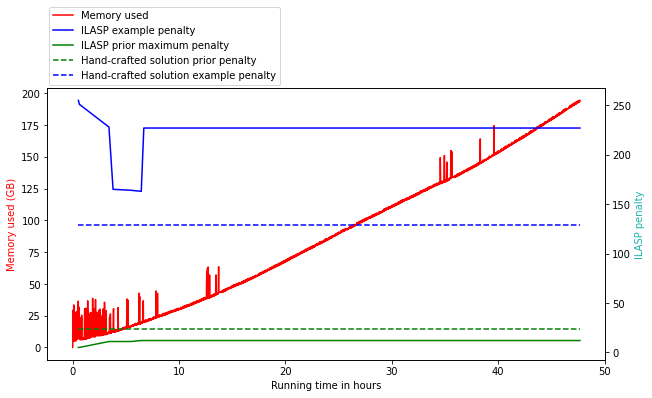
\includegraphics[width=\textwidth]{solving-nlp-tasks-logically/atomisation_memory_vs_best_score.png}
\label{atomisation-memory-graph}
\end{figure}

% INSERT reference Mark theiss% 
ILASP can theoretically find the optimal solution for any noisy task, and the search space represents the hand-crafted solution in full. 
So, we expect the complete run of the task to produce at least as good of a solution as the hand-crafted one.
However, this expectation does not hold within the memory and time constraints available for the \textbf{atomisation} task as shown in \ref{atomisation-memory-graph}.

Observing the maximum prior penalty, we can see that the learner is stuck attempting simple solutions for the duration of the task run. 
The hand-crafted solution uses 24 predicates, whereas the learner never attempted a solution with more than 14 predicates.
This behaviour is quite unlike the one observed for the \textbf{generalisation} task and may even suggest a presence of a bug.

\section{Implementation}

This section presents the implementation design for the learning task and the dependencies used in this code.

\subsection{Atomisation/generalisation procedure}

% TODO: Alessandra feedback: Cut-up this diagram in two one for learning time and one for inference time. With this approach we can replace it to the appropriate report sections.
% TODO: Alessandra feedback: Use ASP Encoder instead of ASP Generator
% TODO: Alessandra feedback: Use Answer Set (Generalised Concept) instead of just Answer Set


\begin{figure}[h]
\caption{Simplified architecture for the concept generalisation part of the CoDEx pipeline.} 
\centering
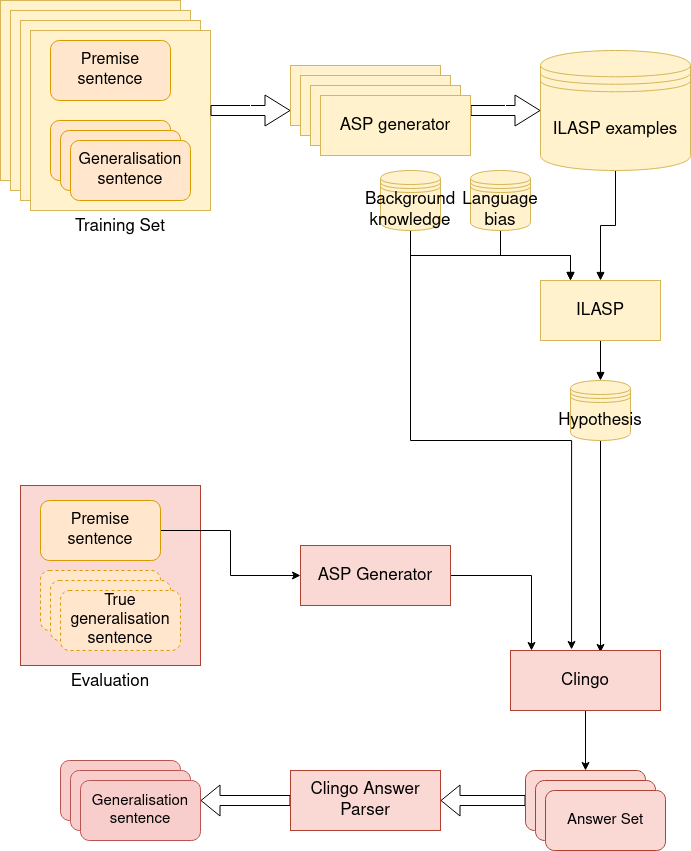
\includegraphics[width=\textwidth]{solving-nlp-tasks-logically/simplified architecture diagram.png}
\label{generalisation-architecture-diagram}
\end{figure}


The architecture diagram of the \textbf{concept generalisation} is shown in \ref{generalisation-architecture-diagram}.
It can be divided into \textbf{learning} and the \textbf{application/evaluation} stage.
The atomisation task uses an almost identical architecture as the \textbf{application/evaluation} stage, where the learned solution is replaced with a hand-crafted one. 
The goal of the \textbf{learning} stage is to learn the hypothesis $H$, which will be able to generalise/atomise any sentence correctly.
Each training example for the learning stage consists of the premise and generalisation sentences provided in CSV format.
The raw examples are written in the following way:

% TODO: Alessandra feedback: This would need to go to either generalisation or atomisation to get the idea of what the data is like.

\begin{center}
\setlength\parskip{0pt}
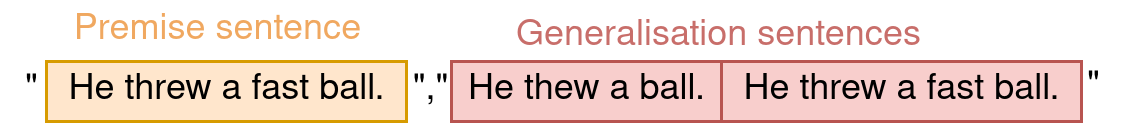
\includegraphics[width=.8\linewidth]{solving-nlp-tasks-logically/raw-generalisation-example.png}
\end{center}

% INSERT spacy/AlunNLP reference
The \textit{ASPGenerator} uses an NLP library to obtain the dependency graph of each sentence, used in the logical representation of an example.

The example files (\textit{ILASP examples} in \ref{generalisation-architecture-diagram}) are persisted since ILASP can only be run as a command line tool.
In addition, the ILASP examples can be split into multiple text files, commonly ten. 
% INSERT condor reference
The split of the files is used to run 10-fold cross validation experiments, parallelised using Condor, a batch processing system.
% TODO: verify this - can be resolved immediately.
The final learned solution (hypothesis $H$), as is the standard practice when doing cross validation, has been produced by training the model with all examples.

% TODO: fix ASP Generator in image
The \textbf{application/evaluation} uses the learned hypothesis in order to split the unknown sentences.
In particular, the process consists of the following stages, visible in \ref{generalisation-architecture-diagram}:
\begin{enumerate}
    \item Conversion to the logical form --- The sentences are converted to the logical form in a manner equivalent to learning encoding. The same module carries out both operations.
    
    % INSERT reference clingo
    \item Answer set solving --- A sentence in the logical form, learned hypothesis and background knowledge are passed to the Clingo answer set solver. Clingo will output all the answer sets of the provided program.
    
    \item Answer parsing --- Each answer set returned corresponds to one generalisation/atomisation sentence. For each \verb+in_generalised_sent+/\verb+in_atomic_sent+ token in an answer set, the actual word corresponding to that token is found. Words are joined in the same order as they appeared in the original sentence. Finally, post-processing techniques (\ref{post-processing-techniques}) are applied to the resulting string to fix possible grammatical issues. 
\end{enumerate}

\begin{example}
Generating all of the generalisations of the sentence \emph{He threw a fast ball.} at test time.

1. Remove . and lowercase all the words in the sentence as a part of pre-processing. The string \emph{he threw a fast ball} is the result of the operations.

2. Convert the sentence to the logical form as shown by the \textbf{example \ref{logical-encoding-example}}.

% INSERT clingo reference
% INSERT next section reference
3. The answer set solver clingo is applied with atoms and predicates existing in the background file, the learned solution file, and the generated predicates.
The construction of the background and the learned solution file will be described in X.

The resulting clingo output is:
\begin{verbatim}
Answer set #1:
{in_generalised_sent(tok0), in_generalised_sent(tok1), 
 in_generalised_sent(tok2), in_generalised_sent(tok3), 
 in_generalised_sent(tok4), in_generalised_sent(tok5)}.
    
Answer set #2:
{in_generalised_sent(tok0), in_generalised_sent(tok1), 
 in_generalised_sent(tok2), in_generalised_sent(tok4), 
 in_generalised_sent(tok5)}.
\end{verbatim}

4. For each answer set generated, we reconstruct a sentence. 
The sentence reconstruction is done by converting each \verb+in_generalised_sent+ token to the back to its string representation.
They are then joined in the same order they originally appeared.

For instance, the \verb_Answer set #2_ converts the tokens with tok0 $\rightarrow$ "he", tok1 $\rightarrow$ "threw", tok2 $\rightarrow$ "a", tok4 $\rightarrow$ "ball".
They are joined to a sentence \textit{he threw a ball}

5. Post-processing clean-up involving truecasing and adding punctuation results in \emph{He threw a fast ball.} and \emph{He threw a ball.} \\
\end{example}
 
\subsection{Post-processing techniques}
\label{post-processing-techniques}

% INSERT reference truecasing
Two post-processing techniques are used to return a grammatically correct sentence: punctuation addition and truecasing.

The \verb_punct_ tags are filtered before logical encoding since the task becomes easier without them.
The punctuation addition adds the punctuation at the end of each solution sentence.
The punctuation added to each atomised/generalised sentence is the same as the punctuation of the original sentence.

% TODO: either reference stack overflow or find how I knew what I needed to capitalise.
Truecasing determines the correct capitalisation where such information is unavailable.
% INSERT https://www.scribbr.com/language-rules/capitalization-rules/
As outlined in X, capitalisation is required for all proper nouns and first words of sentences. 
The latter is simple to implement, while the former heavily relies on a part-of-speech tagger. 
% INSERT reference Penn Treebank
The implementation uses a POS tagger that assigns Penn Treebank tags to words which capture whether a noun is proper using \textit{NNP} (proper noun, singular) and \textit{NNPS} (proper noun, plural) tags.


% Clear page so that the diagram can be inserted
\clearpage 

% Briefly mention dependencies
% INSERT tags for all dependencies
\subsection{Dependencies}

% Modify this paragraph to talk about why we chose Answer Set Programming as a paradigm.

A logic-based learning paradigm was chosen for this task due to the limited number of examples available.
There were two required characteristics that the chosen ILP system needed to have: 
\begin{enumerate}
    \item It needed to be general enough to learn multiple solutions from a single premise.
    \item It must handle noise since the dataset is unlikely to be 100\% accurate.
\end{enumerate}
ILASP \cite{RefWorks:RefID:18-law2020ilasp} is the most advanced system at the moment satisfying these properties.
For this reason, we needed an answer set solver to use solutions ILASP produced. 
Clingo \cite{RefWorks:RefID:22-clingo} is by far the most mature answer set solver at the moment.

Any non-ASP code is written in \textbf{Python} due to the maturity of the NLP libraries for that language. \\
In particular, we used the \textbf{Spacy} -- one of the most famous NLP libraries at the time of writing.
It is used to determine part-of-speech tags of the tokens, create a dependency parse tree for a sentence and split sentences. \\
Finally, \textbf{PyFakeFS}, a library which mocks the file system, was used for testing purposes.

\section{Evaluation}

\subsection{Metrics}


% TODO: Alessandra feedback: talk about metrics such as Jaccard@5, Jaccard@0.1 where the former allows Levensthein distance to be <= 5 for the result to be correct and the latter allows Edit distance to be <= 0.1 length

Both atomisation and generalisation problems had a set of solutions of unknown size.
A needed metric would give a higher score if two sets are very similar compared to those far apart.

There were three metrics which we measured for that reason: Jaccard Index, Set-Recall, and Set-Precision:

$Jaccard \; Index$ is a metric defined as follows:
\begin{itemize}
   \item $Jaccard(A, B) = \frac{card(A \cap B)}{card(A \cup B)}$, where $card$ represents set cardinatlity, $A$ a set containing the true solutions, while $B$ contains the predicated solutions.\\
\end{itemize}
It measures the overlap between the two sets.
 
$Set-Precision$ and $Set-Recall$ are defined in the similar manner as the $Precision$ and $Recall$ in the classification context:
\begin{itemize}
    \item $Set-Precision(A, B) = \frac{card(A \cap B)}{card(B)} = \frac{number \; of \; correctly \; predicted \; sentences}{number \; of \; predicated \; sentences}$
    \item $Set-Recall(A, B) = \frac{card(A \cap B)}{card(A)} = \frac{number \; of \; correctly \; predicted \; sentences}{number \; of \; correct \; sentences} $ 
\end{itemize}
where $card$ represents set cardinality, $A$ a set containing true solutions, while $B$ contains predicated solutions. 
These two metrics help better understand the type of errors the model is making.


% Contains more sophisticated metrics if needed.
% That would ideally involve a similarity in number of produced solutions and similarity of the elements themselves.
% 
% Due to this reason, a single number would have been hard to interpret since it would make it unclear what kinds of mistakes the model is making. 
% For that reason, the evaluation is done with metrics which work with sets with possibly reduced notion of element equality.
% 
% 
% These metrics are also evaluated in a slightly relaxed manner using Levensthein distance.
% $Jaccard\text{-}k$ is a notation used in this report where two elements of a set are equal if their Levensthein distance is less or equal $k$.
% The same notational trick is used for $Recall\text{-}k$ and $Precision\text{-}k$.
% 

% TODO: Alessandra feedback: Show a learned H because it is interpretable (might want to do some analysis there)
\subsection{Concept Generalisation}
\label{concept-generalisation-results}

\subsubsection{Cross-validation results}

Due to only 130 examples available, we are using 10-fold cross validation to get the results for this chapter.
In addition, to complete the execution with 16 GB of RAM, the computation is cut after 12 hours of running time (as argued in \ref{avoiding-oom-errors}).

The results are summarised in the table below:

\begin{center}
\centering
\begin{tabular}{ |M{3cm}||M{3cm}|M{3cm}|M{3cm}|  }
 \hline
 \multicolumn{4}{|c|}{Summary of results} \\
 \hline
  &Jaccard Index&Precision&Recall\\ 
 \hline
 Training  & 0.92 $\pm$ 0.00 & 0.95 $\pm$ 0.00 & 0.95 $\pm$ 0.00 \\
 Test & 0.85 $\pm$ 0.03 & 0.89 $\pm$ 0.02 & 0.89 $\pm$ 0.02 \\
 \hline
\end{tabular}
\end{center}

Overall, the results are relatively high, with >85\% test average.
Looking into more detail the types of mistakes the final model makes, they can be subdivided into three groups:

% INSERT how often each occurs for one solution % 
\begin{itemize}
    \item Genuine errors --- The learned solution fails to produce the examples correctly.
    \item Borderline errors --- The solution does not precisely match the provided gold standard. However, the produced solution might have been made by another data annotator. So, it is probably sufficiently good.
    % INSERT reference: https://spacy.io/models/en#en_core_web_lg
    \item Parser errors --- The dependency parser is imperfect, which can be seen as the cause of some incorrect solutions. For example, a more accurate transformer parser labels \textit{foul ball} as a compound of nouns, whereas the CPU-optimised one used in the project believes \textit{foul ball} has an adjective. The reported LAS accuracy of the CPU-optimised parser is 0.9.
\end{itemize}

Finally, in all experiments, $Set$-$Precision$ and $Set$-$Recall$ were very similar, meaning that missing a solution and producing an incorrect one was similarly likely.


\subsubsection{Comparison with the Manually-Engineered Solution}

The hypothesis was learned and engineered on a subset of the MLB-V2E dataset \cite{RefWorks:RefID:16-2021automatic}.
% INSERT CUB reference
We compare their performance on the MLB-V2E dataset and a subset of the CUB-bird dataset, an out-of-domain dataset.
The former dataset consists of 120 generalisation examples, while the latter has 100 samples.

The results are summarised in tables below:

\begin{center}
\begin{tabular}{ |M{3cm}||M{3cm}|M{3cm}|M{3cm}|  }
 \hline
 \multicolumn{4}{|c|}{In Domain Dataset} \\
 \hline
 \hline
  &Jaccard Index&Precision&Recall\\ 
 \hline
 Hand-crafted $H$ & 0.79 $\pm$ 0.03 & 0.86 $\pm$ 0.03 & 0.80 $\pm$ 0.03 \\ 
 Learned $H$ & 0.92 $\pm$ 0.02 & 0.95 $\pm$ 0.02 & 0.94 $\pm$ 0.02 \\
 \hline
\end{tabular}
\end{center}

\begin{center}
\begin{tabular}{ |M{3cm}||M{3cm}|M{3cm}|M{3cm}|  }
 \hline
 \multicolumn{4}{|c|}{Out Of Domain Dataset} \\
 \hline
 \hline
  &Jaccard Index&Precision&Recall\\ 
 \hline
 Hand-crafted $H$ & 0.71 $\pm$ 0.04 & 0.72 $\pm$ 0.03 & 0.83 $\pm$ 0.04 \\ 
 Learned $H$ & 0.83 $\pm$ 0.03 & 0.84 $\pm$ 0.03 & 0.86 $\pm$ 0.03 \\ 
 \hline
\end{tabular}
\end{center}

As expected, the performance is higher with the in-domain dataset.
The out-of-domain dataset evaluation leads to a ~10\% Jaccard Index reduction for both methods. 
The drop is a result of the distribution shift between the two datasets.
In particular, one of the main reasons for the drop in performance is the lack of accounting for the \verb_acomp_ tag (e.g. tag between \textit{is} and \textit{red} in \textit{A bird is red}).
It barely occurs in the MLB-V2E dataset, so both solutions fail to account for it.



\subsection{Atomisation}

% INSERT reference to atomisation learning%
There is no cross-validation evaluation of the ILASP output due to a poor solution being learned and high computation requirements.
However, the best-learned solution is still compared to the hand-crafted one to showcase how far it is from the manually generated one.
To better showcase the poor performance of the learned solution, simple $H$, a hypothesis which always returns the sentence in full, is introduced.

\subsubsection{Comparison of the Learned and Manually Generated Solutions}

The results averages and standard errors are presented in the tables below:

\begin{center}
\begin{tabular}{ |M{3cm}||M{3cm}|M{3cm}|M{3cm}|  }
 \hline
 \multicolumn{4}{|c|}{In Domain Dataset} \\
 \hline
 \hline
  &Jaccard Index&Set-Precision&Set-Recall\\ 
 \hline
 Simple $H$ & 0.18 $\pm$ 0.04 & 0.18 $\pm$ 0.04 & 0.18 $\pm$ 0.04 \\ 
 Hand-crafted $H$ & 0.55 $\pm$ 0.04 & 0.61 $\pm$ 0.04 & 0.63 $\pm$ 0.04 \\ 
 Learned $H$ & 0.38 $\pm$ 0.04 & 0.42 $\pm$ 0.04 & 0.43 $\pm$ 0.04 \\ 
 \hline
\end{tabular}
\end{center}

% TODO: Alessandra feedback: Ale suggested the name empty H, but it may not be completely correct.
% TODO: Alessandra feedback: Discuss number more, what does 0.09 mean essentially
% TODO: Alessandra feedback: Include snippet of the data that have certain characteristics, for example when elaborating on what doesn't work 

\begin{center}
\begin{tabular}{ |M{3cm}||M{3cm}|M{3cm}|M{3cm}|  }
 \hline
 \multicolumn{4}{|c|}{Out Of Domain Dataset} \\
 \hline
 \hline
  &Jaccard Index&Set-Precision&Set-Recall\\ 
 \hline
 Simple $H$ & 0.06 $\pm$ 0.02 & 0.06 $\pm$ 0.02 & 0.06 $\pm$ 0.02 \\ 
 Hand-crafted $H$ & 0.51 $\pm$ 0.04 & 0.55 $\pm$ 0.04 & 0.57 $\pm$ 0.04 \\ 
 Learned $H$ & 0.09 $\pm$ 0.02 & 0.11 $\pm$ 0.03 & 0.11 $\pm$ 0.03 \\ 
 \hline
\end{tabular}
\end{center}

The hand-crafted solution vastly outperforms the learned one, with a 45\% Jaccard Index improvement.
Nevertheless, even the hand-crafted solution displays a lot of room for improvement as the Jaccard index value is at only 0.55.

A significant hurdle for the hand-crafted solution were the sentences with relative clauses. 
For example, the sentence:
\begin{lstlisting}
The pitcher threw the ball which was outside. 
  $\rightarrow$ The pitcher threw the ball. The ball was outside.
\end{lstlisting}
requires that ends of the splitting tag be in the same atomic sentence, which clashes with the existing core atomisation idea (\ref{hand-crafting-the-atomisation-solution}).


The out-of-domain dataset results in a 0.04 Jaccard Index drop for the hand-crafted hypothesis.
However, that dataset seems better suited for the \verb+splitting_tag+ logic used since the sentences presented were less grammatically complex.
The sentences mainly contained conjunctions with sub-clauses rarely appearing.
The poor result comes from splitting the sentences with multiple conjuncts, which were unaccounted for in the hand-crafted solution.

The learned solution performs terribly on the out-of-domain dataset.
There is no conclusive evidence that it consistently outperforms the simple hypothesis, as there is an overlap between the respective $Jaccard$-$Index$ values.

Finally, in all experiments, $Set$-$Precision$ and $Set$-$Recall$ values were similar, meaning that missing a solution and producing an incorrect one was similarly likely.

